\chapter{Introduction}
\label{sec:ch1}

The following thesis will explore the compensation of third-order resonances in the Fermilab Recycler Ring. Consequently, the structure of this work starts out by summarizing the dynamics of charged particles in a storage ring such as the RR. This \hyperref[sec:ch1]{first chapter} summarizes single particle dynamics with the help of exponential Lie operators and moves forward to introduce a relevant concept of collective beam dynamics: the space charge tune shift. This theoretical overview gives segue into the \hyperref[sec:ch2]{second chapter} of this thesis, where the Recycler Ring is introduced and described in detail. Motivation for the compensation of third order resonances is given in this chapter under the framework of current and future operation of the RR. With the basic physics concepts and the description of the machine put in place, the \hyperref[sec:ch3]{third chapter} describes in full detail the scheme and experiments developed in order to compensate third order resonances at low intensities. Before moving to explore the Recycler Ring at high intensities, \hyperref[sec:ch4]{chapter four} provides an interlude in order to show a series of experiments done at the CERN PS Booster. These experiments explore the use of advanced optimization algorithms in the aid of compensating multiple resonance lines simultaneously. Coming back to Fermilab, \hyperref[sec:ch5]{chapter five} showcases the studies and experiments done at high intensities in the RR in order to understand the interplay between the compensation of resonance lines and space charge effects. Finally, \hyperref[sec:ch6]{chapter six} brings down the curtain by providing some general conclusions and future work stemming from this thesis. For now, let this first chapter introduce some relevant concepts.

\section{Lie Maps in Accelerator Physics}

The most basic element of a particle accelerator can be thought of as a black box. This black box takes some single charged particle with initial transverse coordinates $\left( x_0,x'_0,y_0,y'_0 \right)$, as defined in a Frenet-Serret coordinate system, and maps them to some final coordinates $\left( x_f,x'_f,y_f,y'_f \right)$. For simplicity, any longitudinal effect will not be taken into account for this analysis, but can be easily incorporated. By gathering the initial coordinates into a vector, i.e. $\vec{X_0} = \left( x_0,x_0',y_0,y_0' \right)$, and doing the same for the final coordinates, i.e., $\vec{X_f} = \left( x_f,x_f',y_f,y_f' \right)$, one can define the mapping $\mathcal{M}$ that relates both vectors, such that:  
\begin{equation}
\label{eq:ch1map}
\vec{X_f}=\mathcal{M}\vec{X_0}.
\end{equation}
For a charged particle inside some accelerator element that can be described using Hamiltonian dynamics, the mapping $\mathcal{M}$ can be understood in terms of Poisson brackets and exponential Lie operators \cite{wolski,todd1,cernthesis1,cernthesis2}.\\
Let $\vec{X} = \left( q_1,p_1,\dots,q_{n},p_{n} \right)$ be a 2n dimensional vector, made from $n$ pairs of canonical coordinates $(q_i,p_i)$ that make up the 2$n$ dimensional phase space. And let two arbitrary functions $f\left( \vec{X};s\right)$ and $g\left( \vec{X};s\right)$ be functions of $\vec{X}$ and $s$, where $s$ plays the role of the independent "time" coordinate. The Poisson brackets $\left[ \bullet , \bullet \right]$ can be defined as:
\begin{equation}
    \label{eq:ch1poisson}
    \left[ f,g \right] = \sum_{i=1}^{n} \frac{\partial f}{\partial q_i}\frac{\partial g}{\partial p_i} - \frac{\partial f}{\partial p_i}\frac{\partial g}{\partial q_i}. 
\end{equation}
Using this definition, one can explicitly write out the Poisson bracket definition for a 4 dimensional phase space described by state vector $\vec{X} = \left( x,x',y,y' \right)$. This reads: 
\begin{equation}
    \label{eq:ch1poisson1}
    \left[ f,g \right] = \frac{\partial f}{\partial x}\frac{\partial g}{\partial x'} - \frac{\partial f}{\partial x'}\frac{\partial g}{\partial x} + \frac{\partial f}{\partial y}\frac{\partial g}{\partial y'} - \frac{\partial f}{\partial y'}\frac{\partial g}{\partial y}. 
\end{equation}\\
The Lie operator $:f:$ acts on some function $g$ and is the adjoint operator of the Poisson bracket operator. Its definition reads:
\begin{equation}
    \label{eq:ch1lie1}
    :f:g = \left[ f,g \right].
\end{equation}
This specific $:\bullet:$ notation allows for a compact notation in order to define the exponential Lie operator. The exponential Lie operator of an arbitrary function $f$ is defined as
\begin{equation}
    \label{eq:ch1explie1}
    e^{:f:}\bullet = \sum_{k=0}^{\infty}\frac{1}{k!}\left( :f: \right)^k \bullet.
\end{equation}
It turns out that for a Hamiltonian system, the mapping of coordinates from $\vec{X_0}$ to $\vec{X_f}$ follows the expression:
\begin{equation}
    \label{eq:liemap1}
    \vec{X_f}=e^{-\ell :H:}\vec{X}\bigg\rvert_{\vec{X}=\vec{X_0}},
\end{equation}
which is known as a Lie Map \cite{todd1}. In this case, $\ell$ corresponds to the integration length of the independent coordinate. For example, for a particle traversing a magnet which has length $L$, the integration length is $\ell = L$. When looking at the one-turn map, the integration length corresponds to the circumference $C$ of the accelerator over an effective Hamiltonian $H_{eff}$. Furthermore, if working with action-angle variables, the integration length $\ell$ would just be the phase advance $\mu$.\\ 

\section{One-turn Map and Normal Form}

The one-turn map $\mathcal{M}_1$ of a circular accelerator is the composition ($\circ$) of mappings from every element in the ring. Choosing an arbitrary initial point at $s=0$ and going around the ring, the one-turn map describes the transformation of coordinates after one turn, i.e., $\vec{X}_{N=1}=\mathcal{M}_1 \vec{X_0}$. This map composition reads:
\begin{equation}
    \label{eq:oneturnmap}
    \mathcal{M}_1=M_{N+1} \circ e^{:h_N:} \circ \dots \circ e^{:h_2:} \circ M_2 \circ e^{:h_1:} \circ M_1 = M_{N+1}e^{:h_N:} \dots e^{:h_2:}M_2 e^{:h_1:}M_1,
\end{equation}
where $M_i$ is the matrix representation of a linear mapping, that does not couple $x-y$ plane, e.g., drift space mapping, quadrupole mapping. On the other hand, the map $e^{:h_i:}$ represents any non-linear mapping that can be found around the machine including coupling elements, e.g., skew quadrupoles, higher order multipole elements.  

\begin{figure}[H]
    \centering
    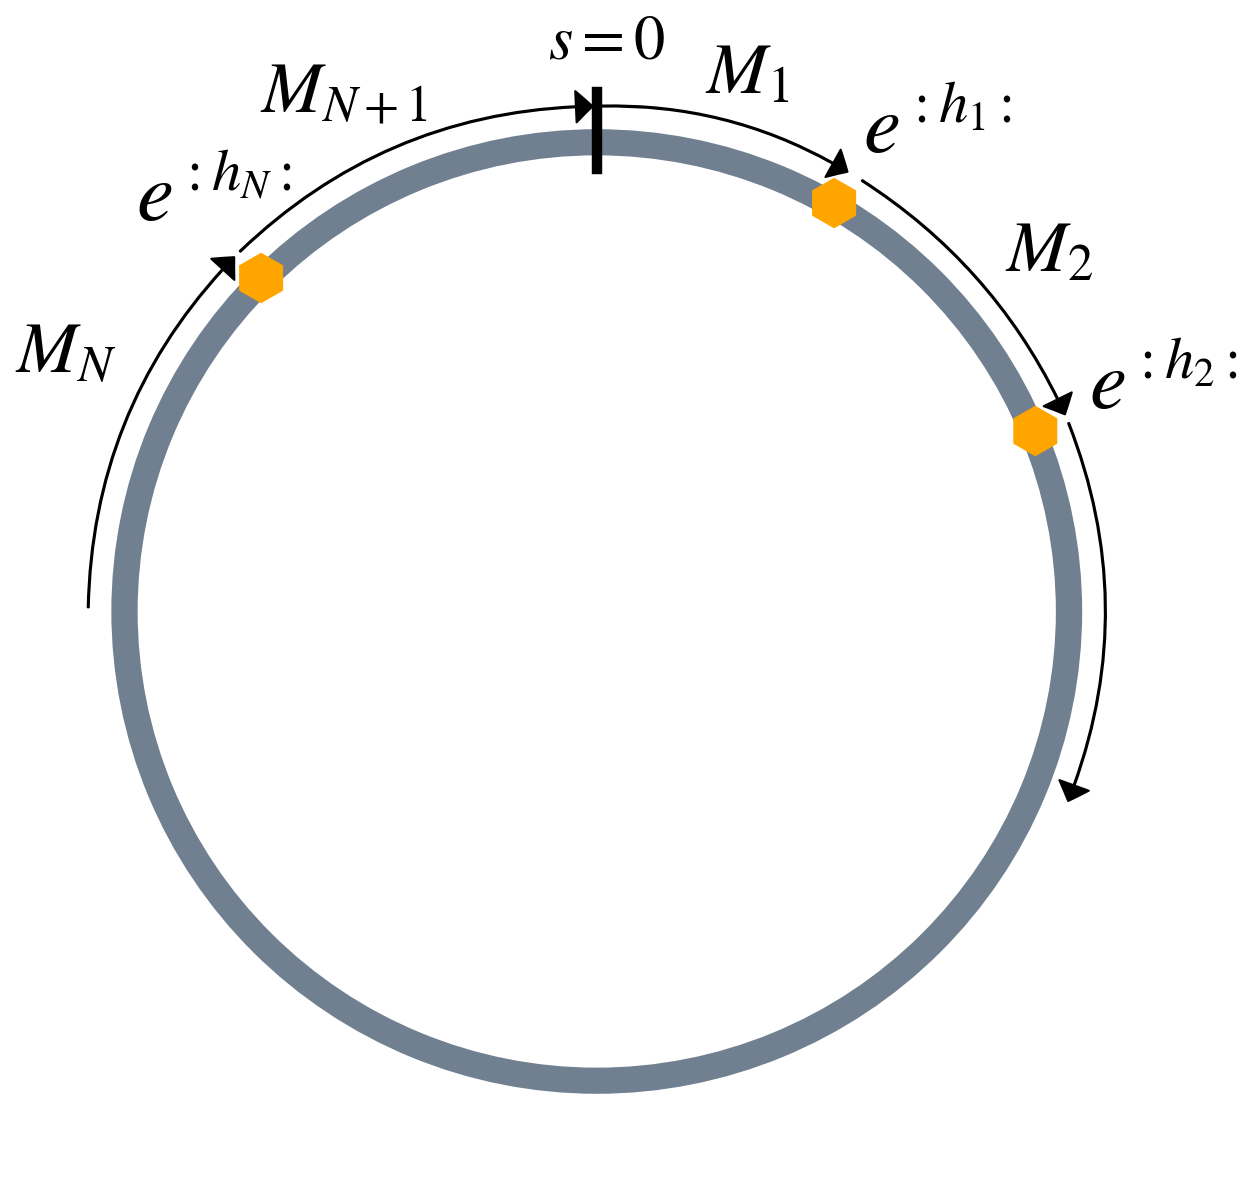
\includegraphics[width=0.7\columnwidth]{chapter1/oneturn.png}
    \caption{Diagram of an arbitrary circular accelerator in order to illustrate the one-turn map.}
    \label{fig:oneturn}
 \end{figure}


\section{Resonances in Circular Accelerators}

\begin{figure}[H]
    \centering
    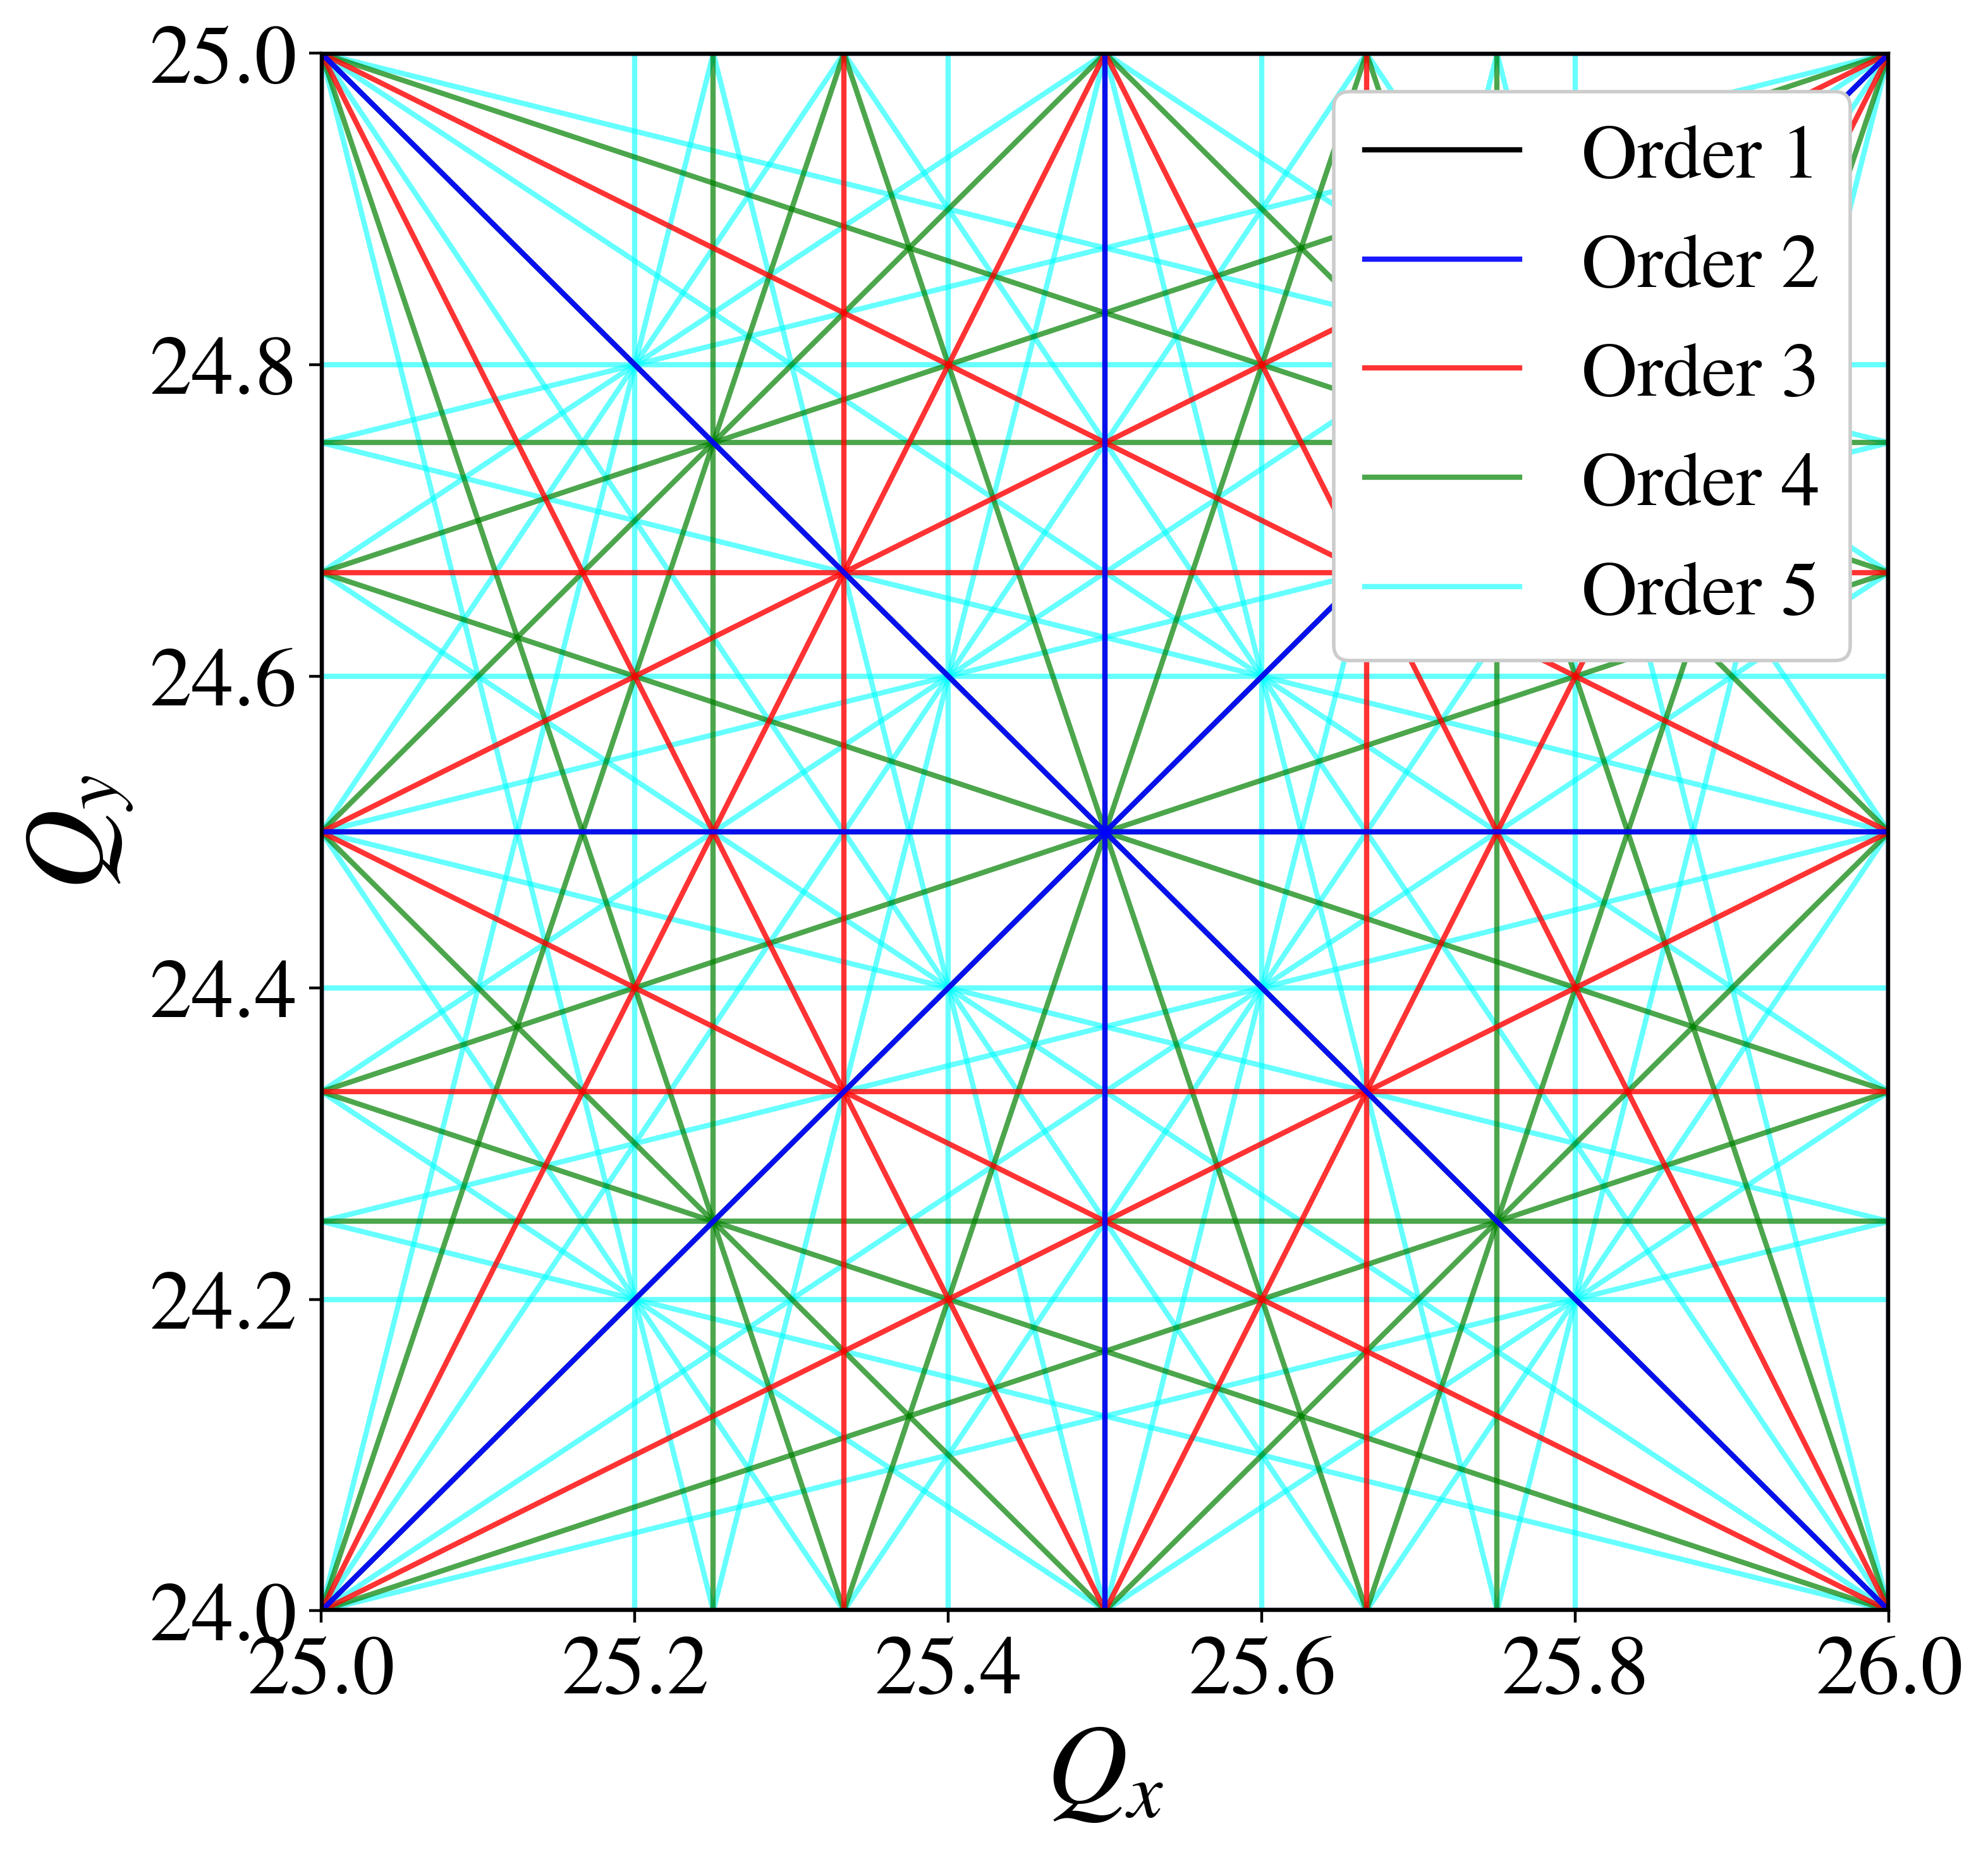
\includegraphics[width=0.8\columnwidth]{chapter1/tunediagram.png}
    \caption{Tune diagram with resonance lines up to fifth order, enclosing the operation point of the Recycler Ring.}
    \label{fig:tunediagram}
 \end{figure}

 \begin{figure}[H]
    \centering
    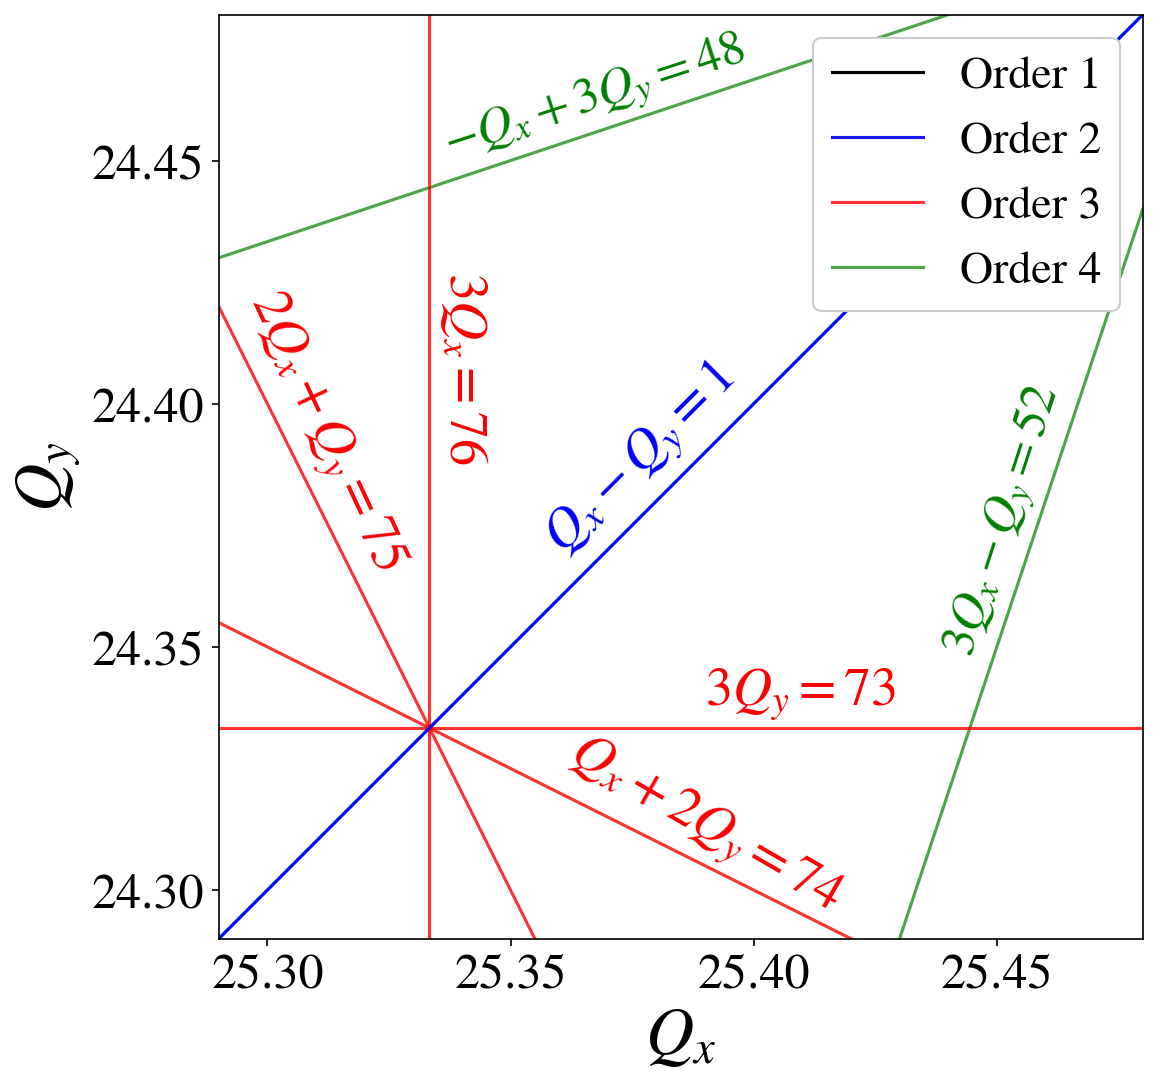
\includegraphics[width=\columnwidth]{chapter1/rrtd.png}
    \caption{Portion of the tune diagram enclosing the operational tunes of the Recycler Ring.}
    \label{fig:rrtd}
 \end{figure}

\section{Resonance Driving Terms}

\section{Space Charge Tune Shift}
